% !Mode:: "TeX:UTF-8"
\chapter{实验与分析}

除了理论的分析结果,本文还关心第四章提出的贪心算法在带有非次模节点的现实中网络的效果。
本文设计了一系列实验,对比了不同网络、不同$\varepsilon$-次模逼近节点个数和不同$\varepsilon$情况下算法的表现并分析了实验结果。
所有的实验都是在一台$128$GB内存、2.4GHz Intel(R) Xeon(R) E5-2620 CPUs、四核$24$线程和$64$位Ubuntu 14.04.1的机器上测试。
本文测试所有的算法都是用C++实现,用g++ 4.8.4编译。
为了节约测试实现,部分算法通过omp多线程实现

\section{实验配置}

\subsection{实验数据}
我们在三个实际网络中执行实验。
第一个网络是{\em Flixster},是美国的一个电影评价社交网站。
每个节点代表一个网站用户,用户间的边代表着用户间的关系。
边上的概率基于主体独立级联模型\cite{barbieri2012topic}(Topic-aware Independent Cascade Model)学习到,
从网络结构和用户间评分的顺序和影响关系基于即极大似然估计学习到边的概率。
Barbieri等人\cite{barbieri2012topic}提供了很多主题的图中边概率,我们采用主题3的$29357$个节点和$174939$有向边。

第二个网络是{\em NetHEPT},是arXiv (http://www.arXiv.org)网站上"High Energy Physics - Theory"主题下的学术合作网站。
许多影响力最大化的相关工作
\cite{Chen2009efficient,chen2010sharpphard,Goyal2011simpath,goyal2012minimizing,mtai2016sigmod}
都用这个网络作为基准去测试算法性能。
在{\em NetHEPT}中,每个节点代表一个作者,每条变代表着作者间曾经合作过的论文。
边的权值代表着作者间合作论文的数量。
{\em NetHEPT}中有$15233$个节点和$31376$条无向边。
在试验中,我们把每一条无向边替换为两条有向边。
在原始网络中,网络中边的值通过weight cascade model\cite{Kempe2003maximizing}设定。
每条有向边$(u,v)$的权值为$c(u,v)/d(v)$,其中$c(u,v)$是$u$和$v$两个作者之间合作发表过的论文数,
$d(v)$是作者$v$发表过的论文数量。

为了评价算法在大型社交网络上的表现,我们采用了{\em DBLP}网络。
{\em DBLP}网络也是一个学术关系合作网络,由Michael Ley维护着。
{\em DBLP}比前两个网络都要大很多,网络中有$654628$个节点和$1990259$条无向边,
是一个十万节点、百万关系的网络。

几个网络数据的信息汇总如表\ref{tab:net_info}所示。
\begin{table}[h]
	\centering
	\caption{网络信息汇总表}
	\label{tab:net_info}
	\begin{minipage}[t]{0.8\textwidth} 
		\centering
		\begin{tabular}{|c|c|c|}
			\hline
			网络  &  节点数   &   边数\\ \hline
			{\em NetHEPT}  &  $15233$   &   $31376$ \\ \hline
			{\em Flixster}  &  $29357$   &   $174939$ \\ \hline
			{\em DBLP}   &   $654628$   &   $1990259$ \\
			\hline
		\end{tabular}\\[2pt]
	\end{minipage}
\end{table}

\subsection{传播模型}
许多学者采用 weight cascade model\cite{Kempe2003maximizing}给边赋值影响概率,
但是在本文我们主要研究通用阈值模型。
我们只考虑线性阈值模型\cite{Kempe2003maximizing},因为直接在次模的阈值函数上运行贪心算法效率很低。
但是线性阈值模型上可以运行TIM算法,利用逆向可达集合的技术算法可以很快输出结果。
更进一步为了构造$\varepsilon$-次模逼近函数,我们给边$(u,v)$赋值为$1/d(v)$。
一个节点每条入边权值一样是为了保证在后面的变换后函数仍然满足单调性。
在这个设定下,阈值函数实际上是一个线性函数$f_v(S) = |S|/d(v)$。

我们根据Backstrom\cite{backstrom2006group}和杨洋\cite{yang2016role}的观测结果构造了下面两种$\varepsilon$-次模逼近函数
\begin{description}
\item[(1)] 幂函数$\frac{|S|}{d(v)}^{\beta}$,$\beta$根据$\frac{1}{d(v)}^{\beta}=\frac{1}{d(v)}(1-\varepsilon)$求出
\item[(2)] $|S| \leq 2$时函数值为$\frac{|S|}{d(v)}(1-\varepsilon)$,$|S| > 2$时函数值为$\frac{|S|}{d(v)}$
\end{description}
第一个$\varepsilon$-次模逼近函数是一个超模函数,这个函数对应了杨洋\cite{yang2016role}在{\em Flickr}网络上观测的结果,
如图\ref{fig:Flickr}所示。
第二个阈值函数在输入大小不超过$2$时有一个向下的掉落,这符合Backstrom\cite{backstrom2006group}现在{\em LiveJounral}网络上的观测结果,
如图\ref{fig:LiveJounral}所示。
为了方便,这两个函数简记为\easso 和\easst ,函数的图像如图\ref{fig:eas12}所示。
\begin{figure}[h]
\centering
	\subfigure[\easso]
	{
		\label{fig:eas1}
		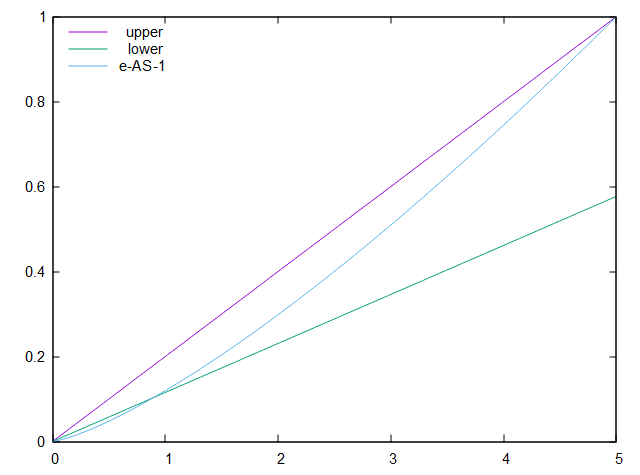
\includegraphics[width=0.35\textwidth]{eas1.png}
	}
    \subfigure[\easst]
	{
		\label{fig:eas2}
		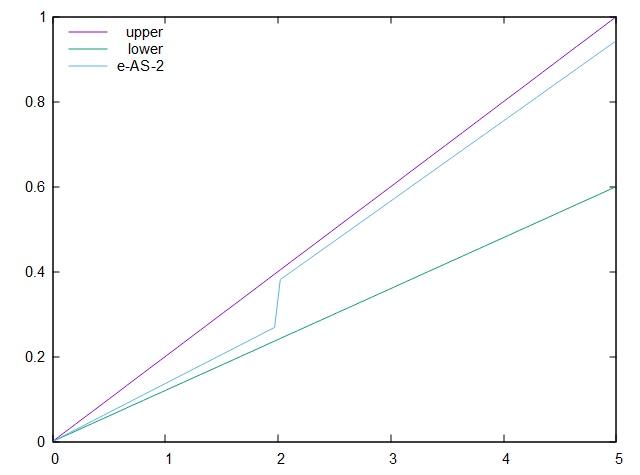
\includegraphics[width=0.35\textwidth]{eas2.png}
	}	
	\caption{Results of IM on {\em NetHEPT} with $\varepsilon=0.2$}
	\label{fig:eas12}
\end{figure}

\subsection{实验算法}
我们测试了本文提出的\textsf{Galg-L}和\textsf{Galg-L}算法,
比较了\textsf{Galg-U}和\textsf{Galg-L}和其他算法在有$\varepsilon$-次模逼近节点图中的表现。
因为最终$\varepsilon$-次模逼近函数的次模上界和下界是线性函数,
所以\textsf{Galg-U}和\textsf{Galg-L}使用TIM算法作为贪心算法,可以称为\textsf{TIM-U}和\textsf{TIM-L}。


\begin{itemize}
\item {\sf TIM-U, TIM-L:}
Tang等人\cite{tang2014newrrset}提出了基于逆向可达集合的{\sf TIM$^+$}算法。
但是{\sf TIM$^+$}不可以直接应用到一般的带有$\varepsilon$-次模逼近节点的图上。
我们把所有的$\varepsilon$-次模逼近阈值函数替换为他们的上届,然后运行{\sf TIM$^+$}算法产生种子集合。
我们称之为{\sf TIM-U},也是第四章提出的算法\ref{alg:Galg_L},算法可产生有近似比保证的输出。
\item {\sf Greedy:} 简单粗暴的在图上根据贪心策略,迭代过程中每一轮选择边际影响力提升最大的节点加入种子集合。
在有$\varepsilon$-次模逼近节点的图中算法没有理论保证,但是通常情况下贪心算法在实际网络效果不错。
\item {\sf High-degree:} {\sf High-degree}计算每个节点的度(degree),然后根据度的降序输出前$k$个节点作为种子节点。
\item {\sf PageRank:} PageRank在度量节点的重要程度时被广泛运用,PageRank的思想是重要的节点会指向重要的节点。
在论文中,边$e=(u,v)$的传递概率被定义为$1/d(u)$,重启概率被设置为$0.15$。
我们用幂方法(power method)计算每个节点的PageRank值,然后输出PageRank值比较高的$k$个节点。
\item {\sf Random:} {\sf Random}随机的输出$k$个节点作为种子。
\end{itemize}

\subsection{实验方法}

数据集提供了网络的结构,我们假设每个节点都有线性的阈值函数。
然后在每次实验中,随机的选取一些入度大于$2$的节点,然后把这些节点的阈值函数变成$\varepsilon$-次模逼近函数,\easso 或者 \easst。
然后调节不同的$\varepsilon$-次模逼近节点个数,$\varepsilon$值的大小,不同的$\varepsilon$-次模逼近函数,然后比较实验结果。
由于贪心算法的运行速度很慢,所以贪心算法的实验只在{\em NetHEPT}上测试。


\section{实验结果}


\subsection{{\em NetHEPT}上实验结果}
第一组实验在{\em NetHEPT}网络上测试,主要是为了对比{\sf TIM-U, TIM-L}算法和{\sf Greedy}算法的表现。
{\sf TIM-U, TIM-L}有理论的近似比保证,但是在图中有大量的$\varepsilon$-次模逼近算法时近似比会很差。
与此相反,尽管影响力函数$\sigma(\cdot)$不是次模函数,
粗暴的根据影响力函数选择边际影响力最大的节点假如种子集合往往能在实际中取得不错的结果。
图\ref{fig:NetHEPT_comp}展示了不同实验设定下每个算法输出种子集合的影响力大小,$1$到$100$种子的结果都被展示了。
图\ref{fig:hept_3000_comp}和图\ref{fig:hept_10000_comp}是有$3000$个\easso 节点的{\em NetHEPT}的测试结果。
可以观察到{\sf TIM-U, TIM-L}比{\sf Greedy}略好一些,不管是在$3000$个还是$10000$个$\varepsilon$-次模逼近节点的图中。
实际上\easso 函数是超模函数,{\sf TIM-U, TIM-L}的表现应该比较差。
{\sf TIM-U, TIM-L}甚至在图中有许多超模节点的图中也打败了{\sf Greedy}算法。

\begin{figure}[h]
\centering
	\subfigure[$3000$ \easso 节点]
	{
		\label{fig:hept_3000_comp}
		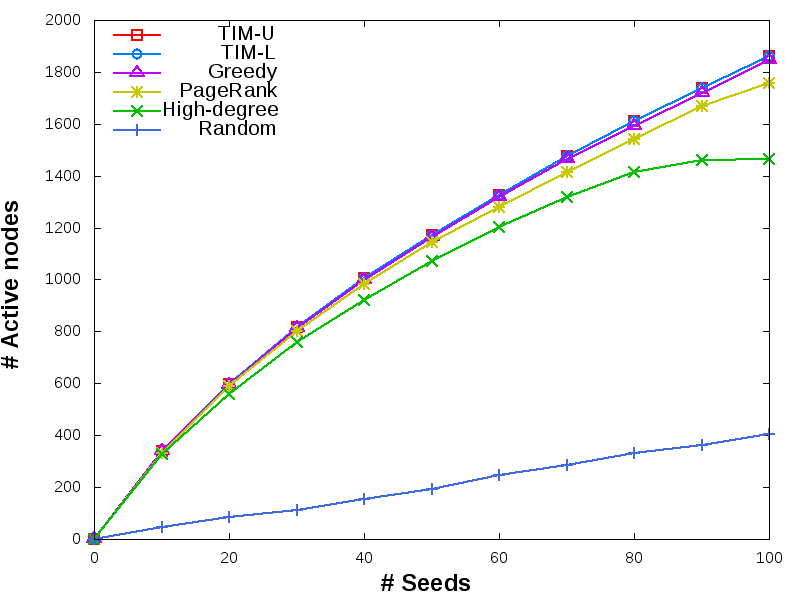
\includegraphics[width=0.425\textwidth]{hept_3000_comp.png}
	}
    \subfigure[$10000$ \easso 节点]
	{
		\label{fig:hept_10000_comp}
		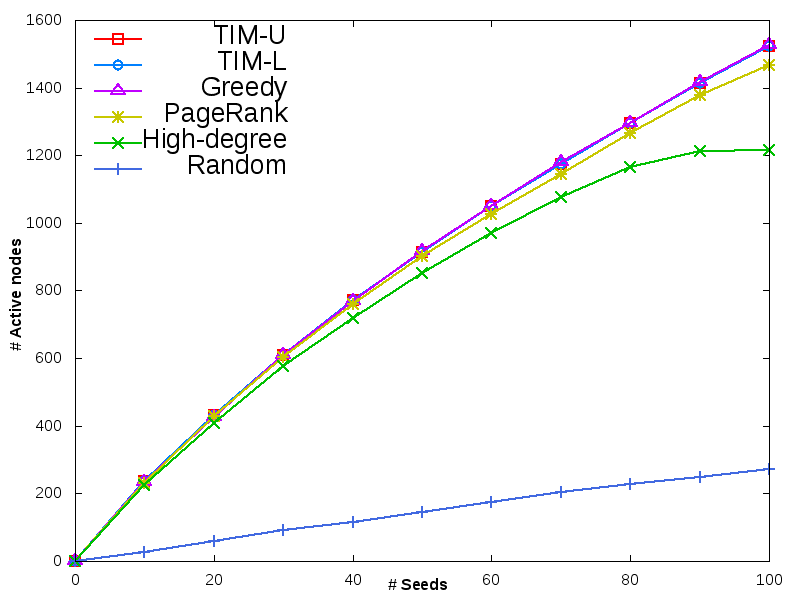
\includegraphics[width=0.425\textwidth]{hept_10000_comp.png}
	}
    \subfigure[$3000$ \easst 节点]
	{
		\label{fig:hept_3000_lt_comp}
		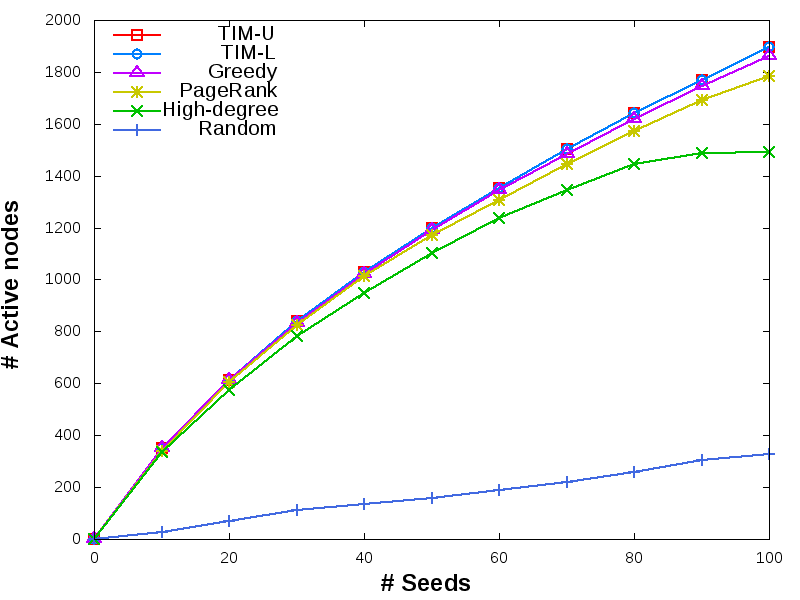
\includegraphics[width=0.425\textwidth]{hept_3000_lt_comp.png}
	}
    \subfigure[$10000$ \easst 节点]
	{
		\label{fig:hept_10000_lt_comp}
		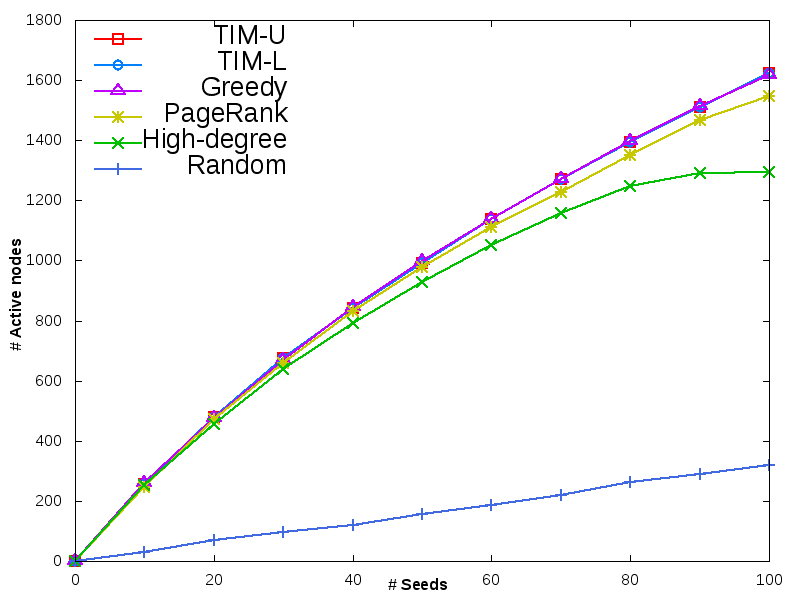
\includegraphics[width=0.425\textwidth]{hept_10000_lt_comp.png}
	}
	
	\caption{{\em NetHEPT}中$\varepsilon=0.2$的结果}
	\label{fig:NetHEPT_comp}
\end{figure}


注意到{\sf TIM-U, TIM-L}和{\sf Greedy}算法在任何设置下都明显打败了其他所有的基准算法。
当种子节点个数$k=100$时,{\sf TIM-U}算法的效果比{\sf PageRank}算法要好$6.1\%$,比{\sf High-degree}要好$27.2\%$。
当在有\easst 节点的图中测试时,图\ref{fig:hept_3000_lt_comp}和图\ref{fig:hept_10000_lt_comp}
中可以看出{\sf TIM-U, TIM-L}算法和{\sf Greedy}算法的表现仍然大幅领先其他算法。
在有\easst 节点的图中,影响力算法的表现比有\easso 节点的图中表现要好一些,这也跟我们期望的一致:
超模函数在$\varepsilon$-次模函数中是最难优化的一类。
因为超模函数和次模函数是相反的概念,完全背离了贪心算法的策略。


另一件值得注意的事是{\sf TIM-U, TIM-L}算法可以在几秒内产生{\em NetHEPT}的种子节点,
但是简单的贪心算法{\sf Greedy}需要跑数周才能输出种子集合,即使是在$24$线程加速的情况下。
图中有非次模节点时,{\sf Greedy}不能使用任何的次模策略进行加速。
但是实验中次模上下届是线性函数,通过逆向可达集合{\sf TIM$^+$}算法极大的缩短了算法运行时间。
我们这里选测线性阈值函数的原因也是为了保证{\sf TIM$^+$}算法可以被应用。
由于{\sf TIM-U, TIM-L}算法的效果基本和{\sf Greedy}算法一致而运行时间又很短,
后文中不再用较大的网络中测试{\sf Greedy}算法的效果。


\subsection{{\em Flixster}上实验结果}

接下来在{\em Flixster}上测试算法效果。
图\ref{fig:Flixster_2}给出了在{\em Flixster}网络中,
包含$\varepsilon=0.2$的$\varepsilon$-次模逼近节点情况下影响力最大化算法的效果。
然后又测试了$\varepsilon=0.4$的设置下影响力最大化算法,结果在图\ref{fig:Flixster_4}中。
观察到{\sf TIM-U, TIM-L}算法在任何设置下都比基准的启发式算法要好很多。
跟{\sf PageRank}算法对比,{\sf TIM-U, TIM-L}算法有在图\ref{fig:Flixster_2}的几组实验中分别有
$30\%,46.3\%,26\%,29.7\%$的提升。
{\sf TIM-U}和{\sf TIM-L}的表现很接近。


\begin{figure}[h]
\centering
	\subfigure[$3000$ \easso 节点]
	{
		\label{fig:flixster_2_3000}
		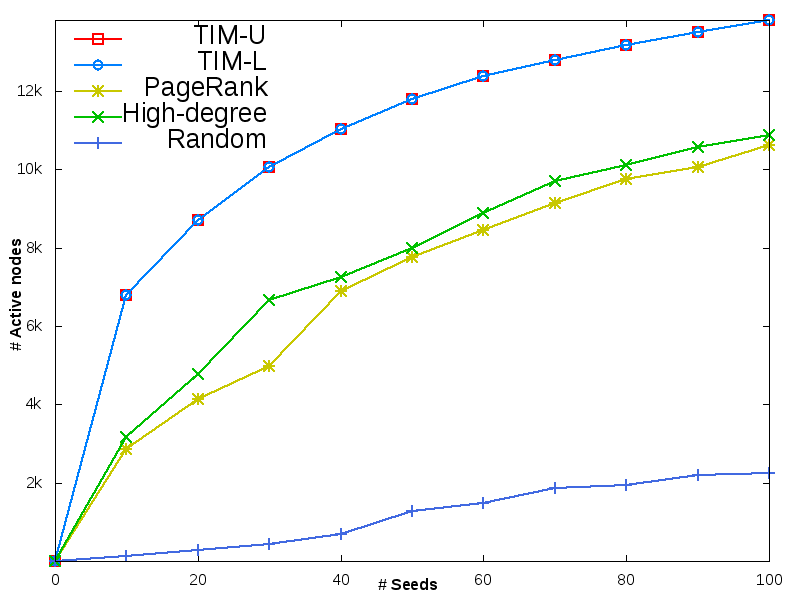
\includegraphics[width=0.425\textwidth]{flixster_2_3000.png}
	}
    \subfigure[$10000$ \easso 节点]
	{
		\label{fig:flixster_2_10000}
		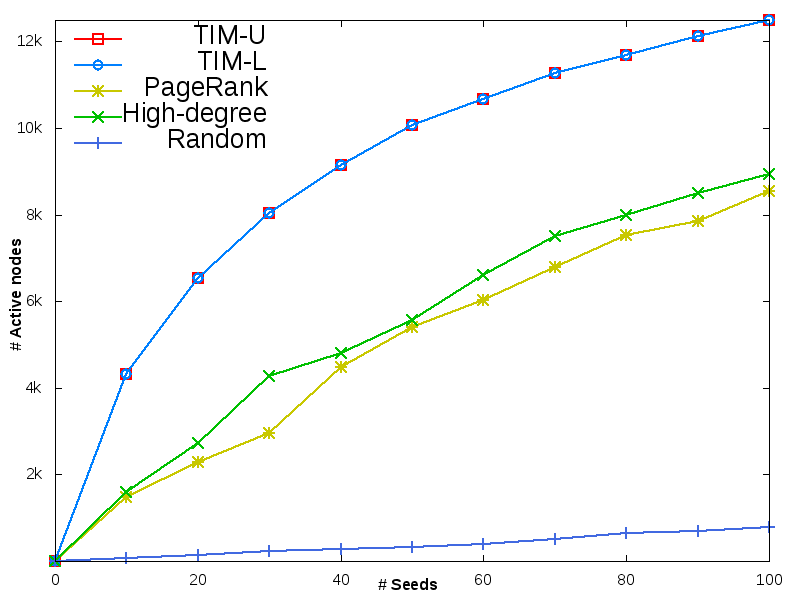
\includegraphics[width=0.425\textwidth]{flixster_2_10000.png}
	}
    \subfigure[$3000$ \easst 节点]
	{
		\label{fig:flixster_2_3000_lt}
		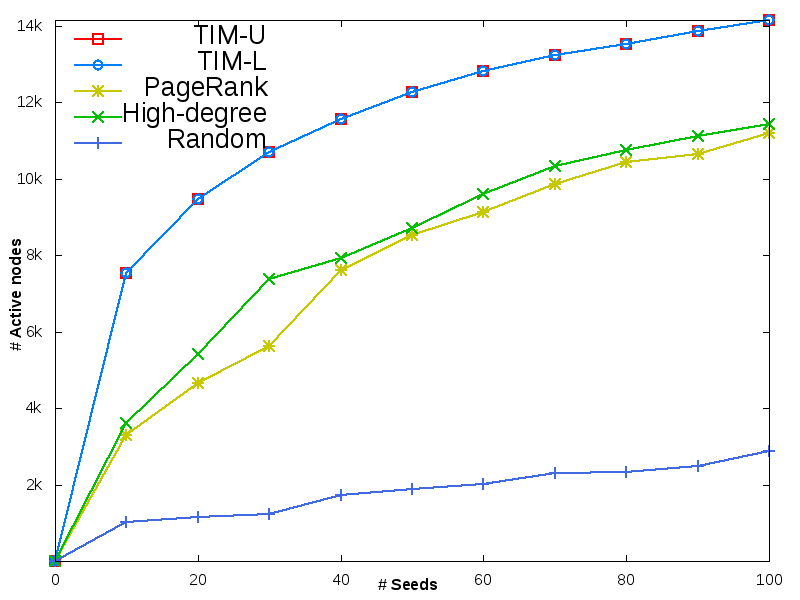
\includegraphics[width=0.425\textwidth]{flixster_2_3000_lt.png}
	}
    \subfigure[$10000$ \easst 节点]
	{
		\label{fig:flixster_2_10000_lt}
		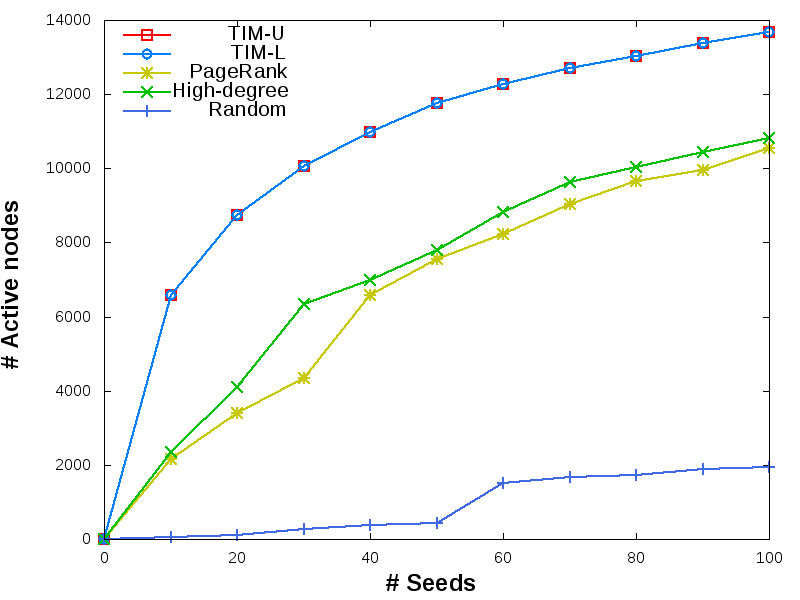
\includegraphics[width=0.425\textwidth]{flixster_2_10000_lt.png}
	}
	\caption{{\em Flixster}中$\varepsilon=0.2$的结果}
	\label{fig:Flixster_2}
\end{figure}

在{\em Flixster}上{\sf TIM-U}和{\sf TIM-L}算法领先基准算法的差距要比{\em NetHEPT}上更大。
这些额外的差距可能是因为{\em Flixster}的网络结构更复杂。
{\em Flixster}图中平均的度是 $5.95$,而在{\em NetHEPT}中只有$2.05$。
在更稠密的网络中,节点可以通过更多的路径被激活,这使得影响力传播过程更为复杂,也传播的更远。
基准算法仅仅关注网络的大体结构,如度、PageRank等,
因而被{\sf TIM-U, TIM-L}这种专门针对影响力优化的算法击败。
当图中有更多的$\varepsilon$-次模逼近节点时,{\sf TIM-U, TIM-L}的相对提升就越大。


\begin{figure}[h]
\centering
	\subfigure[$3000$ \easso 节点]
	{
		\label{fig:flixster_4_3000}
		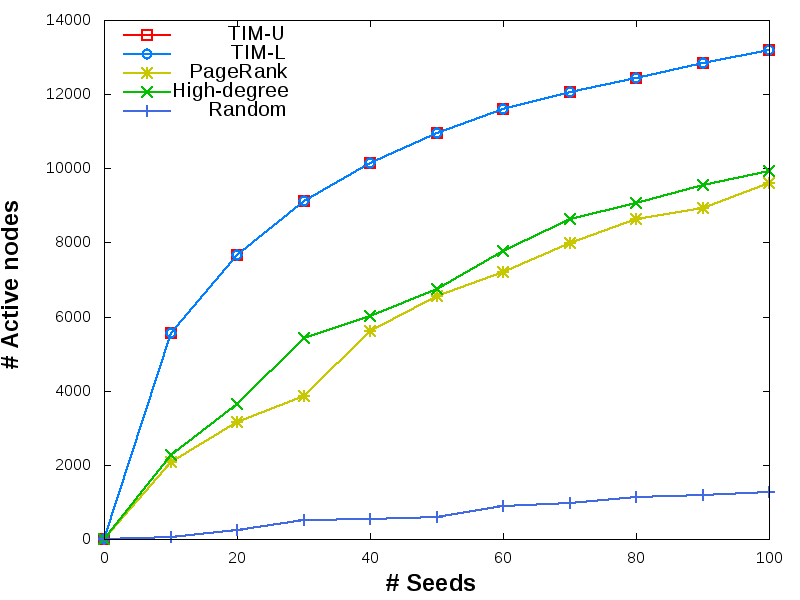
\includegraphics[width=0.425\textwidth]{flixster_4_3000.png}
	}
    \subfigure[$10000$ \easso 节点]
	{
		\label{fig:flixster_4_10000}
		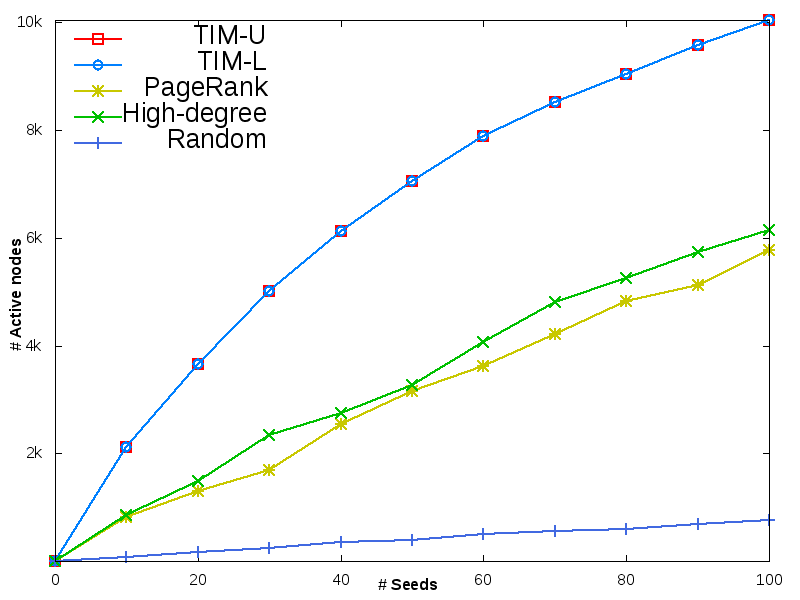
\includegraphics[width=0.425\textwidth]{flixster_4_10000.png}
	}
    \subfigure[$3000$ \easst 节点]
	{
		\label{fig:flixster_4_3000_lt}
		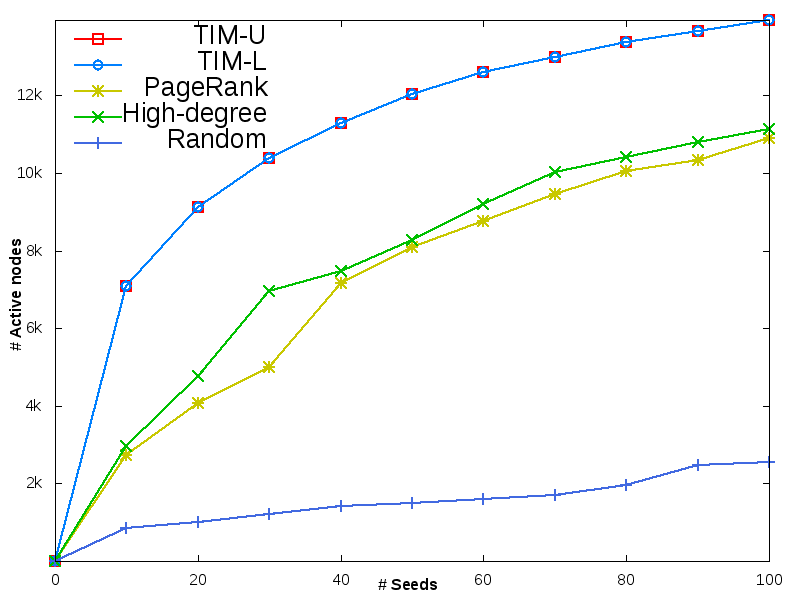
\includegraphics[width=0.425\textwidth]{flixster_4_3000_lt.png}
	}
    \subfigure[$10000$ \easst 节点]
	{
		\label{fig:flixster_4_10000_lt}
		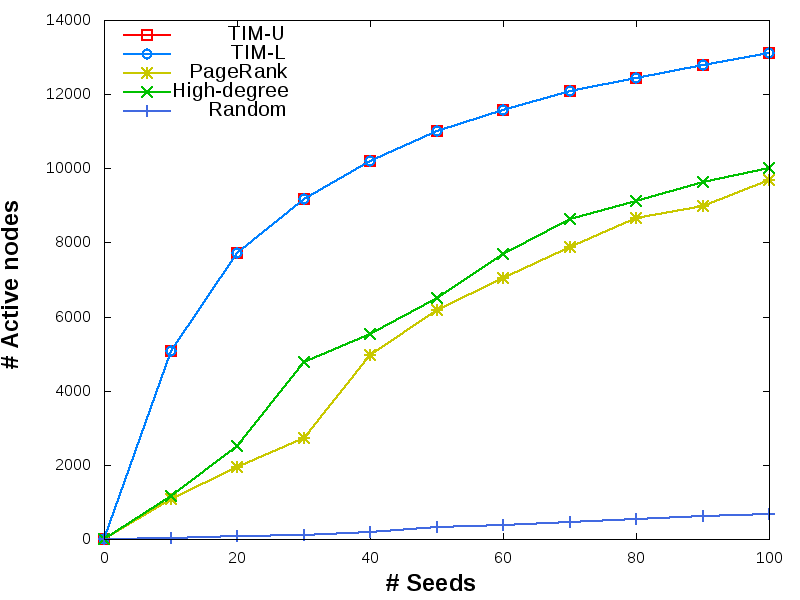
\includegraphics[width=0.425\textwidth]{flixster_4_10000_lt.png}
	}
	\caption{{\em Flixster}中$\varepsilon=0.2$的结果}
	\label{fig:Flixster_4}
\end{figure}

当$\varepsilon$被设置为$0.4$时,也就是$\varepsilon$-次模逼近函数偏离次模更远的时候,
图\ref{fig:Flixster_4}中展示出{\sf TIM-U}相对应于{\sf PageRank}算法分别有$37.6\%,74.2\%,28\%,35.6\%$的提升。
注意到{\sf TIM-U}算法和{\sf PageRank}算法的差距随着$\varepsilon$的增加也增大了。
总的来说在{\em Flixtser}数据集,{\sf TIM-U,TIM-L}相对于其他基准算法有很大优势,
$\varepsilon$-次模逼近节点个数越多,$\varepsilon$越大,优势越大。



\subsection{{\em DBLP}上实验结果}

接下来又测试了节点个数最多的{\em DBLP}网络。
在{\em DBLP}网络上的测试结果如图\ref{fig:dblp_2_1}、图\ref{fig:dblp_2_2}和图\ref{fig:dblp_2_3}所示。
我们分别选用了$10000$、$100000$和$200000$个节点作为$\varepsilon$-次模逼近节点来测试算法的效果。
在{\em DBLP}中仍然可以观测到,{\sf TIM-U}和{\sf TIM-L}是表现最好的算法。
在较大的网络中,{\sf PageRank}和{\sf High-degree}的表现也相当不错,
仅仅在影响力大小上落后{\sf TIM-U,TIM-L}算法$2.6\%$。
我们推测这是因为{\em DBLP}网络中有很多度很大的节点,这些节点对应着在学术圈很活跃的科学家和研究员。
一旦这些节点被激活,影响力会有明显的提升,这也许是{\sf PageRank}和{\sf High-degree}表现亮眼的原因之一。



\begin{figure}[h]
\centering
	\subfigure[$10000$ \easso 节点]
	{
		\label{fig:dblp_2_10000}
		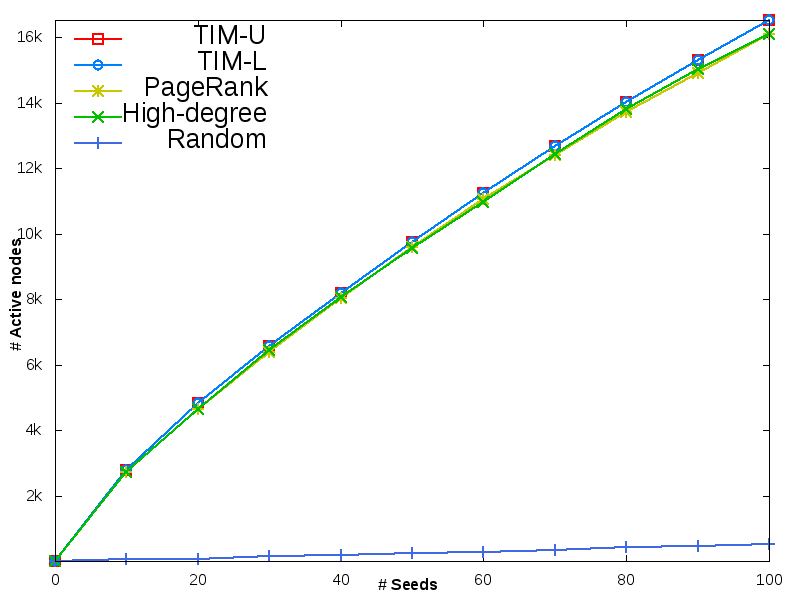
\includegraphics[width=0.425\textwidth]{dblp_2_10000.png}
	}
    \subfigure[$10000$ \easst 节点]
	{
		\label{fig:dblp_2_10000_lt}
		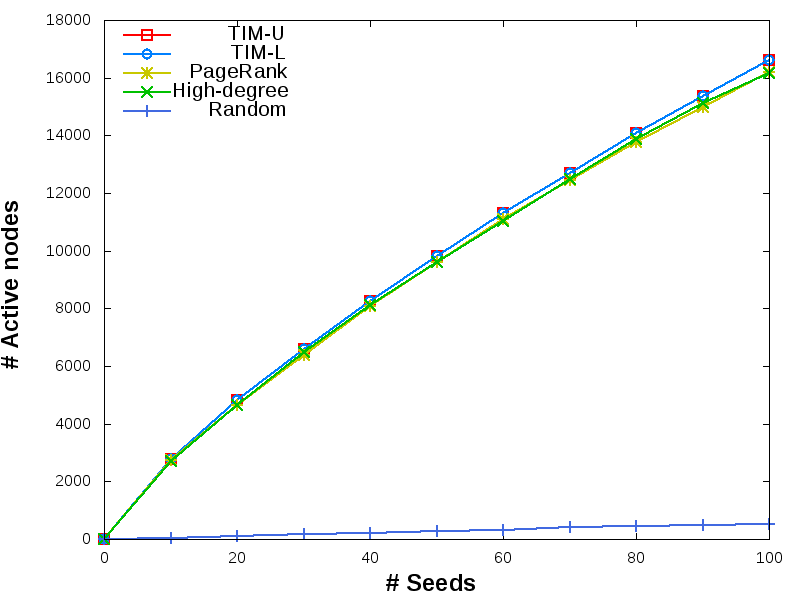
\includegraphics[width=0.425\textwidth]{dblp_2_10000_lt.png}
	}
	\caption{{\em DBLP}中$\varepsilon=0.2$的结果1}
	\label{fig:dblp_2_1}
\end{figure}

\begin{figure}[h]
\centering
    \subfigure[$100000$ \easso 节点]
	{
		\label{fig:dblp_2_100000}
		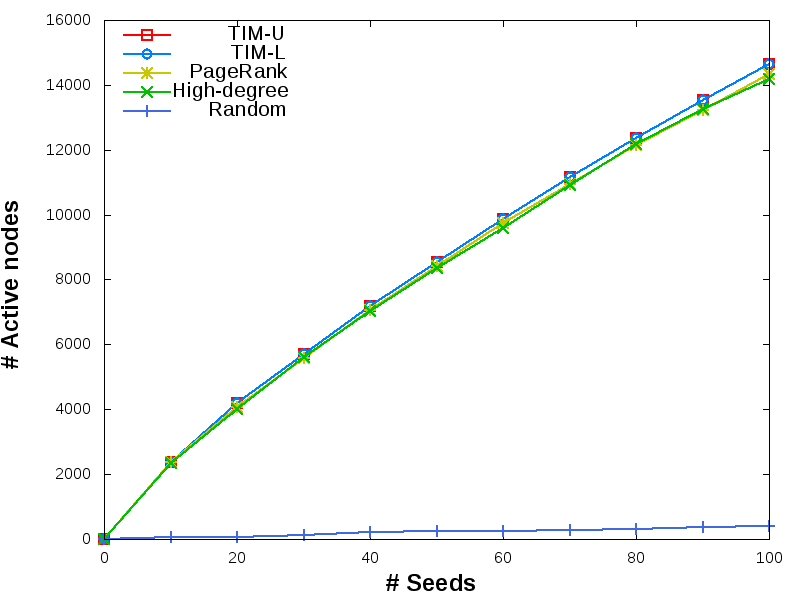
\includegraphics[width=0.425\textwidth]{dblp_2_100000.png}
	}
    \subfigure[$100000$ \easst 节点]
	{
		\label{fig:dblp_2_100000_lt}
		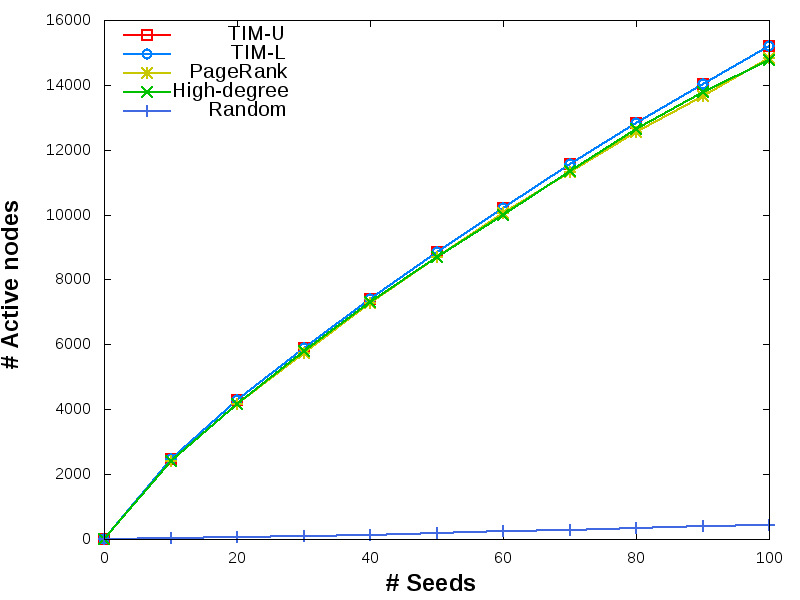
\includegraphics[width=0.425\textwidth]{dblp_2_100000_lt.png}
	}
	\caption{{\em DBLP}中$\varepsilon=0.2$的结果2}
	\label{fig:dblp_2_2}
\end{figure}

\begin{figure}[h]
\centering
	\subfigure[$200000$ \easso 节点]
	{
		\label{fig:dblp_2_200000}
		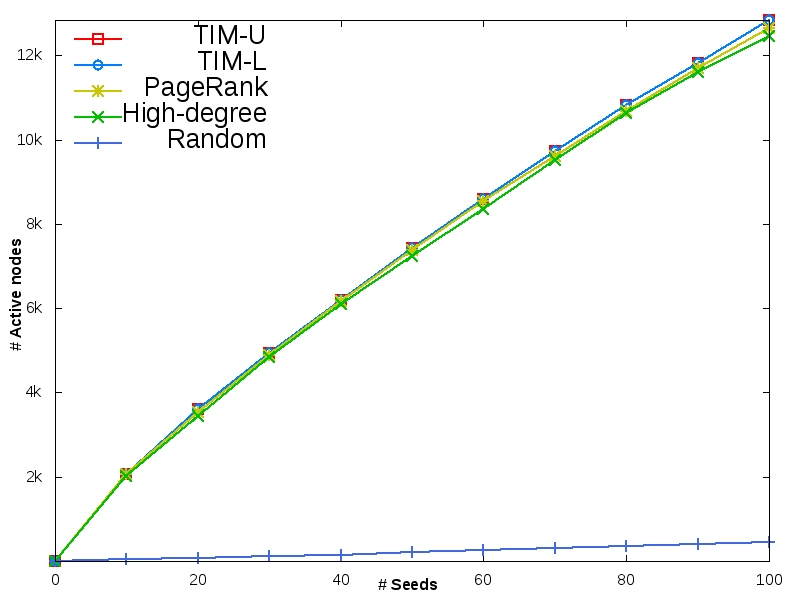
\includegraphics[width=0.425\textwidth]{dblp_2_200000.png}
	}
	\subfigure[$200000$ \easst 节点]
	{
		\label{fig:dblp_2_200000_lt}
		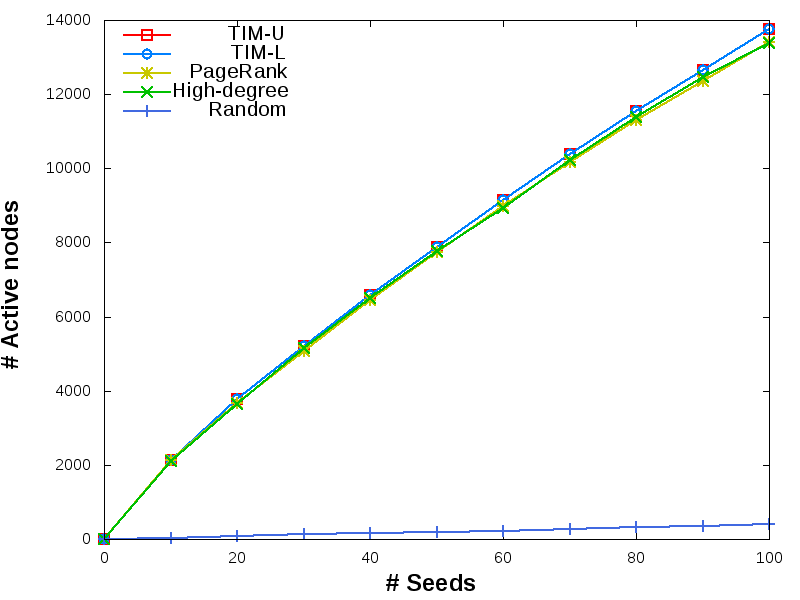
\includegraphics[width=0.425\textwidth]{dblp_2_200000_lt.png}
	}
	\caption{{\em DBLP}中$\varepsilon=0.2$的结果3}
	\label{fig:dblp_2_3}
\end{figure}

{\em DBLP}网络中,即使加入了$200000$个$\varepsilon$-次模逼近节点,
{\sf TIM-U}和{\sf TIM-L}是依然可以表现很好。
这说明我们的算法不仅仅只是在$\varepsilon$-次模逼近节点较少时有较好的理论近似比保证。
算法的设计思路虽然简单,通过转变为次模问题来优化,但是在真实的网络中,算法的表现很好,同时运行时间也可以接受,
$\varepsilon$-次模逼近节点数量的增加没有让{\sf TIM-U}和{\sf TIM-L}表现很差。


\section{本章小结}
本章实现了第四章提出的近似算法\textsf{Galg-U}和\textsf{Galg-L},
并且在真实的社交网络数据{\em NetHEPT}、{\em Flixster}和{\em DBLP}上测试对比了算法和其他基准影响力最大化算法效果并分析了实验结果。
6.1节主要介绍实验的基本配置,介绍了三个网络的基本信息和要对比的算法,然后介绍了如何进行对比。
6.2节分别介绍了{\em NetHEPT}、{\em Flixster}和{\em DBLP}三个真实的网络数据上算法的表现,
\textsf{Galg-U}和\textsf{Galg-L}的效果和\textsf{Greedy}持平,但是运行时间很短。
而且在$\varepsilon$-次模逼近节点较多时算法依然能击败基准算法。





